\chapter{Описание моделей и методов}

В этой главе будут описаны модели и методы, используемые в разработанной системе исправления опечаток. С исходным кодом можно ознакомиться в репозитории, посвященном бакалаврской работе: \url{https://github.com/Mr-Geekman/bd-research}.

\section{Общая схема модели}

Модель состоит из трех модулей:
\begin{enumerate}
	\item модуль генерации кандидатов;
	\item модуль выбора позиции;
	\item модуль выбора исправления.
\end{enumerate}

Опишем общий алгоритм и роль каждого модуля:
\begin{enumerate}
	\item Подготовка:
	\begin{enumerate}
		\item Токенизация.
		\item Нормализация.
		\item Инициализация <<черного списка>> позиций.
		\item Генерация кандидатов для каждого токена и списка признаков к нему при помощи соответствующего модуля.
	\end{enumerate}
	\item Итерации исправления до срабатывания критерия останова или достижения максимального установленного числа итераций:
	\begin{enumerate}
		\item Поиск лучшей позиции для исправления и проверка критерия останова при помощи модуля выбора позиции.
		\item Выбор лучшего исправления в выбранной позиции при помощи модуля выбора исправления.
		\item Изменение текущего предложения в соответствии с предыдущим шагом.
		\item Обновление <<черного списка>> позиций для следующей итерации.
	\end{enumerate}
\end{enumerate}

Теперь разберем отдельные элементы.

\subsection{Токенизация}

На данный момент можно выделить три основных вида токенизации:
\begin{enumerate}
	\item пословная --- токенами являются слова;
	\item посимвольная --- токенами являются отдельные символы;
	\item подсловная --- токенами являются части слов.
\end{enumerate}

Первый тип является самым базовым. Возможных токенов очень много, а потому если это множество как-то ограничивать, то проблемой может стать наличие несловарных слов.

Второй тип не имеет проблем с неизвестными токенами, но при этом весьма сложен в обработке, так как теперь токенов стало гораздо больше на один и тот же объем текста.

Последний вид является промежуточной формой между первыми двумя. Частые слова являются отдельными токенами, а несловарные можно получить из отдельных частей. Таким образом, удается комбинировать преимущества первых двух методик. К примерам алгоритмов, реализующих такой вид токенизации, можно отнести BPE \cite{Gage1994} и WordPiece \cite{Devlin2019}.

В рамках нашей задачи целью является исправление слов на словарные, а потому будем использовать первый тип. Кроме того, это позволит получать консистентные результаты с алгоритмом проверки, так как он тоже оперирует словами.

В качестве алгоритма токенизации была выбрана портированная на язык Python версия токенизатора Moses: \url{https://github.com/alvations/sacremoses}.

\subsection{Нормализация}

Нормализация предложений включала в себя две операции: приведение слов к нижнему регистру, замена буквы <<ё>> на букву <<е>>.

Это не значит, что информация о регистре была окончательно потеряна. В модуль генерации кандидатов передается текст в оригинальном регистре. Тем не менее, все последующие модули работают с уже полностью нормализованным текстом.

Обработка пунктуации не производилась заранее, а отдавалась на откуп модулям.

\subsection{<<Черный список>> позиций}

Это список позиций, которые нельзя выбирать в качестве исправляемых. Он выполняет две функции: 
\begin{enumerate}
	\item Изначальная блокировка некоторых позиций. 
	
	Было решено не исправлять слова, написанные с большой буквы или большими буквами, если они находятся не на первой позиции. Во-первых, таких слов оказалось достаточно мало, а во-вторых, это часто имена собственные или аббревиатуры, про которые сложно сказать, правильно они пишутся или нет.
	
	\item Временная блокировка некоторых позиций.
	
	Предположим, модуль выбора позиции выбрал некую позицию, а затем модуль выбора исправления решил оставить изначальное написание. Если не поместить выбранную позицию в <<черный список>>, то на следующей итерации все повторится. В таком случае, будем помещать выбранную позицию в <<черный список>> до тех пор, пока в предложении не произойдет какое-то исправление, которое может изменить контекст и результат работы модулей.
\end{enumerate}

\section{Модуль генерации кандидатов}

Рассмотрим подробнее модуль поиска кандидатов. Как было указано выше, он отвечает за поиск кандидатов для исправления и генерацию их признаков для каждого токена в предложении.

Общая схема поиска заимствована из статьи <<Automatic spelling correction for Russian social media texts>>\cite{Sorokin2016}. Модуль состоит из трех подмодулей, которые находят кандидатов разными способами:
\begin{itemize}
	\item на основе расстояния Дамерау-Левенштейна;
	\item на основе фонетического кодирования;
	\item на основе вручную закодированных соответствий.
\end{itemize}

Помимо этого, в списке кандидатов обязательно присутствует текущий токен, даже если он отсутствует в словаре. 

Модулю необходим словарь для осуществления поиска. Было решено взять объединение словарей Хагена \cite{Hagen} и wiktionary \cite{Wiktionary} для русского языка, включающее около 2.36 млн. словоформ.

Рассмотрим каждый подмодуль подробнее.

\subsection{Поиск на основе расстояния Дамеарау-Левенштейна}

Модуль был заимствован из библиотеки DeepPavlov \cite{Burtsev2015}. На основе заданного словаря строится ациклический конечный автомат при помощи минимизации префиксного бора. При получении запроса осуществляется алгоритм  A-star \cite{Hart1968} с использованием $h_2$-эвристики из статьи <<Fast approximate string matching with finite automata>> \cite{Hulden2009}.

Для обработки ошибки удаления пробела (при исправлении необходимо вставить пробел), автомат дополняется ребрами из всех конечных состояний в начальное с меткой пробела. Это позволяет при получении словарного слова вставить пробел и продолжить поиск. 

Итого, при выполнении поиска кандидатов для токена извлекаются все словарные слова и группы словарных слов, разделенных пробелами, на расстоянии Дамерау-Левенштейна, не превышающем некоторой фиксированной константы.

\subsection{Поиск на основе фонетического кодирования}

Алгоритмы фонетического кодирования --- это алгоритмы, которые на основе правил произношения преобразуют слова в кодирующий их текст таким образом, что коды близких по произношению слов похожи или совпадают.

Первым представителем подобных алгоритмов является алгоритм SoundEx \cite{Russell1917} \cite{Russell1922}. Существует и множество других алгоритмов, некоторые из которых приспособлены для русского языка. Хороший обзор существующих методов представлен в статье <<Обзор алгоритмов фонетического кодирования>> \cite{Vichovanetch2018}.

В своей модели мы будем использовать алгоритм из лучшего решения SpellRuEval, так как в нем есть несколько особенностей, полезных для исправления опечаток. Каждой букве ставится в соответствие свой фонетический класс согласно таблице \ref{table:phonetic_codes} (нумерация с пропусками кодов 2 и 4 сохранена из оригинальной статьи). 

\begin{table}[h]
	\begin{center}
		\caption{Соответствие букв и их фонетических кодов.}
		\label{table:phonetic_codes}
		\begin{tabular}{|c|c|c|c|c|c|}
			\hline
			\textbf{Код} & \textbf{Буквы} & \textbf{Код} & \textbf{Буквы} & \textbf{Код} & \textbf{Буквы}  \\
			\hline
			1 & а, о, ы, у, я & 8 & г, к, х  & 13 & з, с  \\
			3 & и, е, ё, ю, я, э  & 9 & л  & 14 & й  \\
			5 & б, п  & 10 & р  & 15 & щ, ч  \\
			6 & в, ф  & 11 & м  & 16 & ж, ш  \\
			7 & д, т  & 12 & н & 17 & ц  \\		
			\hline
		\end{tabular}
	\end{center}
\end{table}

Кроме того, есть несколько правил, согласно которым фонетический класс может меняться:
\begin{enumerate}
	\item все гласные после \textit{ь, ъ, щ, ч, й} переходят в класс 3;
	\item все гласные после \textit{ш, ж, ц} переходят в класс 1;
	\item сочетания \textit{тс, тьс, тъс} переходят в класс 17;
	\item выбрасывается \textit{т} после сибилянтов и перед согласной (например, для обработки слова \textit{грустный});
	\item в последовательностях из одинаковых классов оставляется лишь один элемент.
\end{enumerate}

У полученного алгоритма есть несколько полезных свойств:
\begin{itemize}
	\item опускается множественное повторение одной гласной, например, слова <<ооочень>> и <<очень>> получат один и тот же код;
	\item не различаются окончания на <<ться>>, <<тся>>, <<цца>>, например слова <<различаться>>, <<различацца>>, <<различатся>> получат один и тот же код.
\end{itemize}

Итого, при выполнении поиска кандидатов для токена достаются все словарные слова, имеющие тот же фонетический код.

\subsection{Поиск на основе вручную закодированных соответствий}

Третий подмодуль для поиска представляет собой таблицу соответствий между токеном и его возможными заменами. Далее опишем процедуру сбора подобных соответствий.

Большая часть соответствий была собрана на основе данных из социальных сетей корпуса <<Тайга>> \cite{Shavrina2017}.  По токенизированным текстам были посчитаны частоты всех несловарных слов. Перебирая слова от самых частых к самым редким было просмотрено около 5000 слов, из которых были составлены 136 соответствий.

Посмотрим на некоторые примеры:
\begin{itemize}
	\item \textit{че} $\rightarrow$ \textit{что};
	\item \textit{ваще} $\rightarrow$ \textit{вообще};
	\item \textit{щас} $\rightarrow$ \textit{сейчас};
	\item \textit{оч} $\rightarrow$ \textit{очень};
	\item \textit{шоб} $\rightarrow$ \textit{чтобы, чтоб, что бы, что б}.
\end{itemize}

Два соответствия были получены на основе обучающей выборки. Их особенность заключается в том, что это словарные слова:
\begin{itemize}
	\item \textit{тока} $\rightarrow$ \textit{только};
	\item \textit{скока} $\rightarrow$ \textit{сколько};
\end{itemize}

Еще 10 паттернов были закодированы на основе опыта общения в социальных сетях. Примеры:
\begin{itemize}
	\item \textit{пж} $\rightarrow$ \textit{пожалуйста};
	\item \textit{мб} $\rightarrow$ \textit{может быть};
	\item \textit{норм} $\rightarrow$ \textit{нормально}.
\end{itemize}

\subsection{Объединение токенов}

Как уже было описано, модуль умеет обрабатывать ошибки <<один ко многим>>, когда один токен надо разбить на несколько, вставив пробел. Тем не менее, в обучающей выборке присутствуют и ошибки типа <<многие к одному>>, когда надо объединить несколько подряд идущих токенов в один или вставить между ними дефис.

Для решения этой проблемы рассматриваются пары подряд идущих токенов, не являющихся знаками пунктуации. Происходит проверка находится ли в словаре результат удаления пробела между ними или замены его на дефис. Если ответ положительный, то рассматриваемая пара токенов становится отдельным токеном. Список его кандидатов состоит из:
\begin{itemize}
	\item приписывания второго токена к элементам списка кандидатов для первого токена;
	\item приписывания первого токена к элементам списка кандидатов для второго токена;
	\item оригинальных токенов, записанных через пробел,
	\item объединения токенов с удалением пробела или вставкой дефиса (в зависимости от того, что нашлось в словаре).
\end{itemize}

Была также предпринята попытка заменить простую проверку удаления пробела или вставки дефиса на полноценный поиск на заданном расстоянии Дамерау-Левенштейна, но это привело лишь к резкому увеличению числа ложных срабатываний, которых и без того было очень много. 

Можно также заметить, что этот механизм скорее всего непригоден для объединения трех и более слов, тем не менее, такой случай был всего один на всю обучающую выборку.

\subsection{Генерация признаков}

Как было описано выше, модуль генерации кандидатов помимо создания списка исправлений также вычисляет признаки для них, которые будут использоваться в следующих модулях. Перечислим генерируемые признаки:
\begin{itemize}
	\item признаки позиции:
	\begin{itemize}
		\item индикатор написания с заглавной буквы;
		\item индикатор написания заглавными буквами;
		\item индикатор написания строчными буквами;
		\item индикатор первой позиции (чтобы можно было как-то отдельно обработать случаи регистров для нее).
	\end{itemize}
	\item индикатор содержания пробела;
	\item индикатор содержания дефиса;
	\item индикатор нахождения при помощи расстояния Дамерау-Левенштейна;
	\item индикатор нахождения при помощи фонетического кодирования;
	\item индикатор нахождения при помощи таблицы соответствий;
	\item индикатор того, что кандидат является результатом комбинирования смежных токенов;
	\item индикатор того, что кандидат является изначальным токеном в данной позиции;
	\item индикатор того, что кандидат является текущим токеном в данной позиции (отличается от изначального, если в позиции произошло исправление);
	\item индикатор принадлежности словарю.
\end{itemize}

Отдельная сложность возникает при объединении токенов. В случае, когда токен дополняется кандидатами другого токена, брались признаки для изменяемого токена. Для объединенного токена сложность составляло лишь вычисление признаков регистра, но этот случай достаточно редкий.

\section{Модуль выбора позиции}

Рассмотрим модуль, предназначенный для выбора позиции исправления и проверки критерия останова.

В основу модуля положено языковое моделирование. Для каждой позиции можно посмотреть вероятности различных кандидатов в ней при проходе текста как слева направо, так и справа налево. Затем эти вероятности можно сагрегировать, получив для каждой позиции и каждого кандидата некоторое число, характеризующее насколько данный кандидат хорошо подходит в данной позиции. На основе этих данных можно сравнить насколько в каждой позиции лучший кандидат превосходит текущего и выбрать позицию, отсутствующую в <<черном списке>> с самым большим разрывом. Такой способ позволяет отдавать приоритет тем позициям, в которых замена может значительнее всего увеличить вероятность. Для проверки критерия останова достаточно посмотреть на полученный разрыв и сравнить его с зафиксированной константой.

Подход можно усложнить, обучив модель, учитывающую помимо вычисленной сагрегированной характеристики и другие параметры, характеризующие позицию. Эта попытка была предпринята, прочитать о ней можно в соответствующем разделе, посвященном экспериментам. Тем не менее, если не обучать модель и зафиксировать языковые модели, то описанный подход требует настроить только способ агрегации и константу критерия останова.

В качестве способа агрегации было решено взять среднее гармоническое. Пусть логарифм вероятности кандидата от левой языковой модели равна $s_l$, а от правой --- $s_r$, тогда итоговый показатель:

\begin{equation*}
	s = \frac{2 s_l s_r}{s_l + s_r}.
\end{equation*} 

К плюсам именно такого метода можно отнести чувствительность к минимальному значению. Если одна из вероятностей окажется сильно меньше другой, то среднее гармоническое отклонится в меньшую сторону сильнее, чем, например, среднее арифметическое. В то же время, реакция на меньшее значение достаточно сглаженная в отличие от функции минимума.

Также следует описать почему при сравнении позиций берется разность между показателями кандидатов. Дело в том, что на выходе языковых моделей мы получаем логарифмы вероятностей, а их разности характеризуют множитель между вероятностями. Было намерение отдавать приоритет тем позициям, в которых вероятность от исправления может повыситься в наибольшее число раз.

Может появиться мысль оценивать не вероятности кандидатов при условии контекста, а вероятности предложений целиком с подстановкой соответствующих кандидатов. Чтобы сравнить этот подход с описанным в самом начале, рассмотрим как их можно реализовывать на примере модели слева направо (для модели справа налево все аналогично). В обоих подходах достаточно проходиться по предложению слева направо и запоминать текущий левый контекст перед рассмотрением очередной позиции. В подходе из начала раздела достаточно перебрать всех кандидатов, а в подходе, работающим с предложениями целиком, потребуется для каждого кандидата посмотреть, как изменится состояние правой части предложения, что может занять гораздо больше времени. Именно поэтому было решено использовать подход, описанный в самом начале.

В качестве предобработки текста перед применением языковых моделей было решено убрать всю пунктуацию. Также следует прояснить, как обрабатывались кандидаты, состоящие из нескольких токенов. Такое могло произойти если в модуле генерации кандидатов сработал механизм объединения или подмодуль поиска на основе расстояния Дамерау-Левенштейна вставил пробел внутри слова. В таком случае, было решено считать логарифмом вероятности кандидата сумму логарифмов вероятностей отдельных слов внутри него.

После вычисления характеристик каждой позиции в список кандидатов, сгенерированных предыдущим модулем, записываются дополнительные признаки:
\begin{itemize}
	\item логарифмы вероятностей от левой и правой языковых моделей;
	\item агрегированные логарифмы вероятностей (среднее гармоническое);
	\item разница агрегированных характеристик рассматриваемого кандидата и текущего кандидата в данной позиции.
\end{itemize}

\subsection{Языковые модели}

В этом подразделе будут описаны использованные языковые модели и процедура их обучения.

Рассматриваемый модуль имеет высокие требования к производительности, а потому было решено использовать $n$-граммные языковые модели, так как они достаточно быстрые в отличие от нейросетевых. Выбор пал на реализацию в библиотеке KenLM \cite{Heafield2011} \cite{Heafield2013}, которая использует модифицированное сглаживание Кнезера-Нея \cite{Chen1996}.

Было решено обучать модели на текстах из корпуса <<Тайга>>. Было отобрано 100 млн. предложений из разных источников. В процессе предобработки тексты переводились в нижний регистр, буква <<ё>> заменялась на <<е>>, пунктуация удалялась. Было получено несколько версий моделей:
\begin{itemize}
	\item 3-граммная модель;
	\item 3-граммная модель без данных из социальных сетей;
	\item 4-граммная модель.
\end{itemize}

\section{Модуль выбора исправления}

Опишем теперь модуль, отвечающий за выбор конкретного исправления в позиции.

\subsection{Выбор исправления на основе BERT}

Модель BERT была предложена в статье <<BERT: Pre-training of deep bidirectional transformers for language understanding>> \cite{Devlin2019}. Одной из задач, используемых для ее предобучения, является маскированное языковое моделирование (MLM от англ. masked language modeling), которое подразумевает предсказание токена не по одностороннему контексту, а по всему окружению. Достигается это за счет того, что модель по архитектуре является энкодером и обрабатывает все предложение целиком. Кажется вполне разумным рассмотреть задачу выбора исправления, как MLM-задачу. Достаточно выбирать самого вероятного кандидата из списка.

При попытке реализовать этот подход требуется решить, что делать в случае, если кандидат представляет из себя несколько токенов, так как токенизация для модели BERT (WordPiece-токенизация) работает на уровне частей слов. Было решено находить логарифм вероятности для каждого WordPiece-токена внутри кандидата, при этом задав остальным подтокенам значение <UNK> (неизвестный токен) и отключив для них механизм внимания. Таким образом, при вычислении вероятности конкретного WordPiece-токена модель будет знать только позиции других токенов, но не будет принимать во внимание их конкретные значения. 

В качестве примера рассмотрим предложение <<это поделанные документы>>, где будет осуществляться ранжирование кандидатов <<поделанные>> и <<подделанные>> для второй позиции. Пример проиллюстрирован на рис.~\ref{ris:bert_scoring}. На первом шаге происходит вычисление логарифмов вероятностей для первых подтокенов, а на втором --- для вторых. Как видим, кандидат <<подделанные>> оказывается лучше, согласно модели.

\begin{center}
	\begin{figure}[h!]
		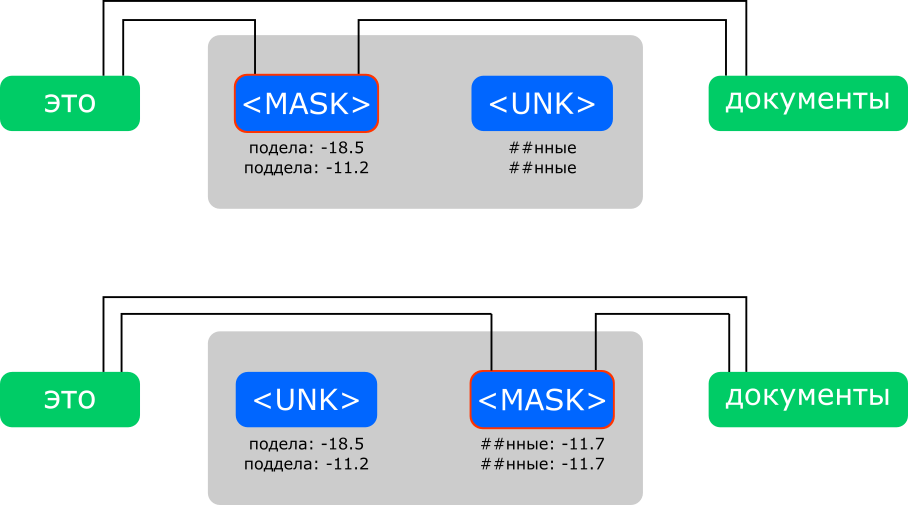
\includegraphics[width=\textwidth]{bert_scoring}
		\caption{Иллюстрация работы ранжирования при помощи BERT.}
		\label{ris:bert_scoring}
	\end{figure}
\end{center}

Возможен и другой подход, когда механизм внимания не отключается для остальных токенов. Во-первых, это может усложнить параллелизацию. Во-вторых, это может привести к слишком сильному влиянию на вероятность других WordPiece-токенов кандидата, а требуется, чтобы кандидат выбирался исходя из окружения, а не частей самого себя.

Таким образом, для каждого кандидата в общем случае получается список логарифмов вероятностей его подтокенов. Для выбора лучшего кандидата требуется сагрегировать значения. Были попытки использовать для этого сумму или среднее.

В целях увеличения производительности был реализован способ группировки MLM-задач, чтобы за один запуск модели проверялось как можно больше кандидатов.
Пусть имеется список из $n$ токенизированных кандидатов одинаковой длины $m$: $[[s_{1 1}, s_{1 2}, \dots, s_{1 m}], \dots, [s_{n 1}, s_{n 2}, \dots, s_{n m}]]$, таких, что $s_{1 i} = s_{2 i} = \dots = s_{n i}$.  Тогда при запуске MLM-задачи для их $i$-го WordPiece-токена будет получаться одинаковый контекст, а значит достаточно будет выполнить запуск модели всего один раз и для каждого кандидата посмотреть на MLM-вероятность. Таким образом, можно группировать MLM-задачи для WordPiece-токенов кандидатов, если кандидаты состоят из одинакового количества подтокенов и все подтокены, кроме рассматриваемых в данный момент, совпадают. Но, как уже было описано выше, при запуске MLM-задачи всем токенам кандидата кроме рассматриваемого в данный момент присваивается значение <UNK>, а значит для группировки MLM-задач достаточно лишь чтобы соответствующие кандидаты состояли из одинакового числа WordPiece-токенов. Такой подход позволяет для любого количества кандидатов длины $m$ выполнить только $m$ запусков модели.

%Для каждой позиции список кандидатов составляют в основном достаточно похожие слова, а значит часто у них будут совпадать WordPiece-токены. Это можно использовать для того, чтобы за один запуск модели проверять как можно больше кандидатов. В самом деле, пусть имеется список из $n$ токенизированных кандидатов одинаковой длины $m$: $[[s_{1 1}, s_{1 2}, \dots, s_{1 m}], \dots, [s_{n 1}, s_{n 2}, \dots, s_{n m}]]$, таких, что $s_{1 i} = s_{2 i} = \dots = s_{n i}$.  Тогда при запуске MLM-задачи для их $i$-го WordPiece-токена будет получаться одинаковый контекст, а значит достаточно будет выполнить запуск модели всего один раз и для каждого кандидата посмотреть на вероятности MLM. Таким образом, можно сгруппировать две MLM-задачи для WordPiece-токенов кандидатов, если кандидаты состоят из одинакового количества подтокенов и все подтокены, кроме рассматриваемых в данный момент, совпадают.

В качестве предобученных моделей BERT для русского языка рассматривались RuBERT \cite{Kuratov2019} и Conversational RuBERT, который представляет из себя дообученный на данных из Интернета RuBERT.

\subsection{Выбор исправления на основе множества признаков}

Оказалось, что предыдущий подход работает не очень хорошо. Точность была совсем невысокой, а значит модели было тяжело выбрать правильное исправление. Появилась мысль, что модели BERT не хватает знаний о том, как совершаются ошибки, то есть требовалась некая модель ошибок. Для этого было решено добавить больше признаков и обучить некую модель ранжирования, которая бы выбирала из списка кандидатов лучшего. 

Опишем используемые признаки:
\begin{itemize}
	\item признаки, вычисленные при генерации кандидатов;
	\item признаки, связанные с языковом моделированием (модуль выбора позиции);
	\item признаки BERT:
	\begin{itemize}
		\item количество WordPiece-токенов;
		\item сумма логарифмов вероятностей для WordPiece-токенов;
		\item среднее логарифмов вероятностей для WordPiece-токенов.
	\end{itemize}
\end{itemize}

Для сбора обучающей выборки была запущена модель, использующая только BERT. Правильные ответы для каждой задачи ранжирования были получены при помощи процедуры выравнивания, использующейся при измерении качества.

В качестве первой модели было решено взять ranking SVM \cite{Joachims2002}, которая представляла из себя линейный SVM \cite{Boser1992}, обученный предсказывать, что один кандидат строго лучше другого на разностях их признаковых векторов. Один кандидат считался лучше другого если являлся правильным ответом. Использовалась реализация алгоритма в библиотеке scikit-learn \cite{Pedregosa2012}.

В качестве второй модели был взят CatBoost  \cite{Dorogush2018}, решающий задачу ранжирования. Этот алгоритм способен улавливать более сложные зависимости, чем SVM, но при этом достаточно хорошо работает при стандартных значениях гиперпараметров. Немного остановимся на принципах его работы. CatBoost --- это алгоритм градиентного бустинга, способный качественно предобрабатывать категориальные признаки и использующий <<забывчивые>> (oblivious) деревья. Их особенность в том, что условие разделения в деревьях выбирается одно на весь уровень, см. рис.~\ref{ris:oblivious_tree}.

\begin{center}
	\begin{figure}[h!]
		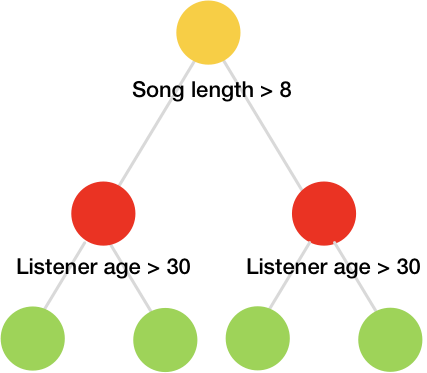
\includegraphics[width=0.5\textwidth]{oblivious_tree}\centering
		\caption{Иллюстрация <<забывчивого>> дерева \cite{CatBoostDocs}.}
		\label{ris:oblivious_tree}
	\end{figure}
\end{center}

В качестве отклика был взят индикатор того, что кандидат является верным ответом. Данные были разбиты на группы, где каждая из них отвечает за конкретную задачу ранжирования по кандидатам в определенной позиции. Были испытаны следующие функции потерь:

\begin{itemize}
	\item \verb|RMSE|.
	
	Решается задача регрессии по предсказанию отклика. Пусть имеются множество задач ранжирования $T$ и множество кандидатов $C$. Тогда если рассматривается конкретная задача ранжирования $t$, то обозначим множество кандидатов, соответствующее ей, как $C_t$. Получим следующую функцию потерь:
	
	\begin{equation*}
		\frac{1}{\sum\limits_{t \in T} |C_t|} \sqrt{\sum\limits_{t \in T} \sum\limits_{c \in C_t} \left( \widehat{y}(c) - y(c) \right)^2}, 
	\end{equation*}
	
	где $\widehat{y}(c)$ --- предсказание модели, а $y(c)$ --- истинный отклик.
	
	\item \verb|QueryRMSE|.
	
	Выражение:
	
	\begin{equation*}
		\frac{1}{\sum\limits_{t \in T} |C_t|} \sqrt{\sum\limits_{t \in T} \sum\limits_{c \in C_t} \left( \widehat{y}(c) - y(c) - \frac{1}{|C_t|} \sum\limits_{\tilde{c} \in C_t} \left( \widehat{y}(\tilde{c}) - y(\tilde{c}) \right) \right)^2}.
	\end{equation*}
	
	Такая функция позволяет не обращать внимания на смещение, так как при ранжировании нам важен порядок, а не абсолютные значения.
	
	\item \verb|PairLogit|.
	
	Эта функция потерь отвечает попарному подходу к решению задачи. Внутри каждой группы $t$ генерируются все возможные пары $P_t$, в каждой из которых первый кандидат лучше, чем второй. Итоговая формула:
	
	\begin{equation*}
		-\sum\limits_{t \in T} \sum\limits_{(c_p, c_n) \in P_t} \ln\left( \frac{1}{1 + \exp\{- (\widehat{y}(c_p) - \widehat{y}(c_n)) \}} \right).
	\end{equation*}
	
	\item \verb|YetiRank|.
	
	Данная функция тоже реализует попарный подход. Подробнее о ней можно почитать в соответствующей статье: <<Winning The Transfer Learning Track of Yahoo!’s Learning To Rank Challenge with YetiRank>> \cite{Gulin2011}.
	
\end{itemize}

Сведения о всех доступных функциях потерь размещены на странице документации: \url{https://catboost.ai/docs/concepts/loss-functions-ranking.html}.
